\chapter{Modelowanie warunków propagacji}
\section{Symulowanie zakłóceń}
\subsection{Wstęp}
Kiedy proces implementacji osiąga pewien stopień zaawansowania nadchodzi czas testowania. 
Oznacza to sprawdzenie projektu pod kątem dostępnych funkcjonalności. 
Prototyp poddany zostaje testom, aby upewnić się czy nie posiada poważnych wad. 
Komercyjne ścieżki rozwoju produktu dopuszczają równoległy proces weryfikacji zarówno u producenta jak u klienta, aby lepiej dostosować się do jego potrzeb \cite{product_dev}. 
System odbiornika tworzony jest wyłącznie dla celów edukacyjnych, dlatego testy zostaną wykonane wyłącznie przez autora projektu. 

W tym rozdziale duży nacisk położony jest na zrozumienie sygnału docierającego do odbiornika. 
Odtworzone zostaną warunki pracy odbiornika poprzez spreparowanie sygnału i poddanie go działaniom zjawisk występujących w kanale radiowym. 
\subsection{Strategia}
Założenia projektowe nie określają jasno wymogów jakościowych i wydajnościowych pracy, a przyjęta strategia weryfikacji ma charakter eksperymentalny. 
Jako pierwsza przetestowana zostanie zdolność odbiornika do eliminacji zakłóceń pojedynczej częstotliwości. 
Scenariusz pokazany na Rysunku \ref{cwmodel} zakłada, że w kanale transmisyjnym sygnał użyteczny silnie interferuje z falą sinusoidalną. 
Dodatkowo występuje nieznaczny dryft częstotliwości sygnału zakłócającego w czasie.
Druga próba to modelowanie kanału jako filtra liniowego o zmiennej w czasie odpowiedzi impulsowej (Rysunek \ref{mpathmodel}). 
Pozwoli to na przetestowanie odbiornika w warunkach zakłóceń związancych z propagacją wielodrogową \cite{indoor_ch_model}.

\begin{figure}[ht]
\centering
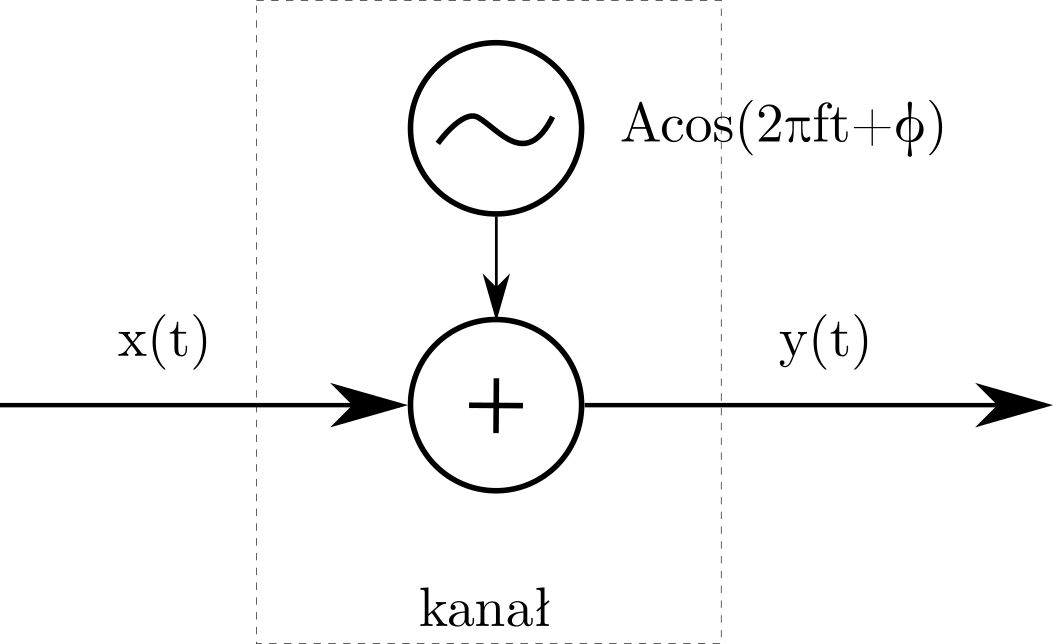
\includegraphics[scale=1.5]{ch_model1.png}
\caption{Model kanału z zakłóceniem pojedynczej częstotliwości}
\label{cwmodel}
\end{figure}

\begin{figure}[ht]
\centering
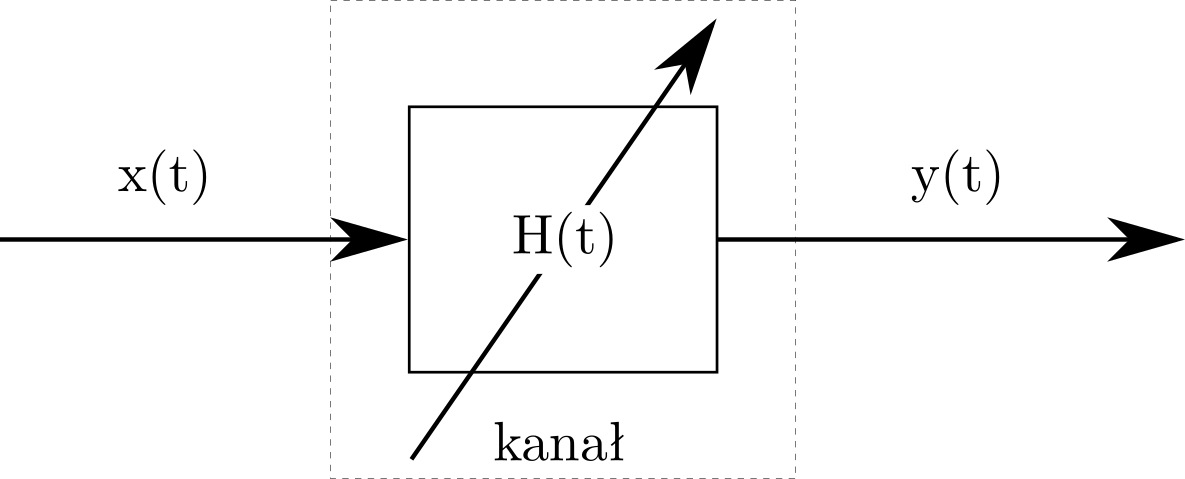
\includegraphics[scale=1.5]{ch_model2.png}
\caption{Model kanału w propagacji wielodrogowej}
\label{mpathmodel}
\end{figure}

\subsection{Zjawisko wielodrogowości}
Występuje wtedy, gdy do odbiornika z wielu kierunków dochodzi ten sam sygnał. 
Fala wydłuża swój tor kiedy odbita od elementów otoczenia zmienia drogę. 
Tym samym każdy sygnał dociera do odbiornika w różnym czasie. 
Fale interferują, wzmacniają się lub osłabiają. 
W określonym czasie przy zachowaniu rozmieszczenia elementów otoczenia, nadajnika i odbiornika, kanał radiowy można traktować jako filtr o odpowiedzi impulsowej $H(t)$.

Jako model kanału z propagacją wielodrogową posłuży blok \texttt{Channel Model}. 
Istotnym argumentem wejściowym dla bloku jest wektor współczynników o długości $M$. Współczynniki przyjmują wartości z zakresu $w_i = [0,1]$, gdzie 0 to brak tłumienia, a dla 1 tłumienie $\to \infty$. Charakterystyka kanału określona jest w przedziale $[-\frac{f_s}{2} + f_c,\frac{f_s}{2} + f_c]$, gdzie $f_s$ to częstotliwość próbkowania, a $f_c$ częstotliwość nośna sygnału. Pasmo kanału dzielone jest na odcinki o szerokości $\frac{f_s}{M}$. Za tłumienie na  $M$ odcinków odpowiada jeden współczynnik. Wartości współczynników powiązane zostały z suwakami do regulacji z panelu graficznego. 


\subsection{Źródła szumów}
\subsection{GnuRadio}
\subsection{Fala ciągła}
\subsection{Szum addytywny}
\subsection{Wielodrogowość}